\section{Introduction}

Ideally we would like mechanistic interpretability to provide guarantees
about the computational process used by a model. We would like features
to be
\begin{enumerate}
	\item causal
	\item disentangled
	\item closed-form
\end{enumerate}
However most existing techniques, such as sparse autoencoders (SAEs),
produce features that can perform arbitrarily badly on these desiderata.
As a dictionary grows, features split into narrower
ones~\cite{bricken2023}, and a narrow feature can absorb a broader one
so that the broader feature fails to fire where it
applies~\cite{chanin2025}, breaking disentanglement. SAE features can't
usually be statically analyzed (though bilinear SAE variants can be).
Sparsity trades off against reconstruction fidelity, limiting the extent
to which features can be used for steering.

Arguably the simplest interpretability technique is a linear probe, and
the simplest control technique is a steering vector. On current
benchmarks both beat features from unsupervised techniques such as SAEs,
with probes ahead on concept detection and the difference of means ahead
on steering~\cite{wu2025axbenchsteeringllmssimple}, but both require
contrastive datasets built around a concept someone has already
named~\cite{burns2023ccs}. In the spirit of MoEfication~\cite{zhang2022}, we
propose a technique based on decomposing a representation space into a
set of contrastive classifiers. Each entry corresponds to a
representative vector (an atom). Inputs are encoded as a series of
classifier assignments and reconstructed from the atoms those
assignments select. This has several advantages over SAEs:
\begin{enumerate}
	\item It effectively gives steering for free: changing a
	head's entry is a steering move.
	\item Outputs are bounded.
	\item The representative vectors admit static interpretation in
	principle, though making this work in practice remains an open
	problem (Section~\ref{sec:prelim-autointerp}).
	\item Feature space is structured.
\end{enumerate}
Figure~\ref{fig:teaser} summarizes the steering behavior of the soft
model, and Section~\ref{sec:prelim} reports our preliminary evaluation,
including where the results do not support these hypotheses.

\begin{figure}[tp]\centering
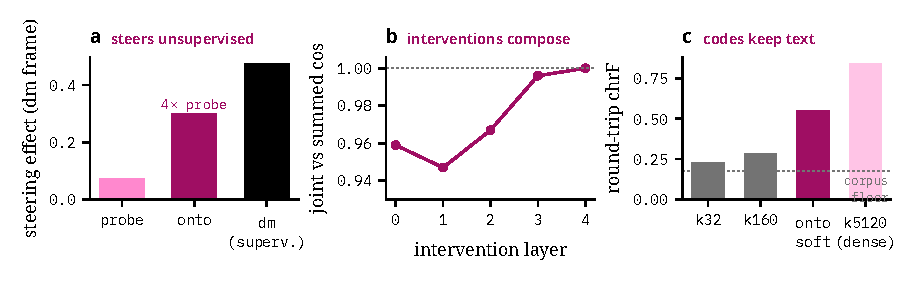
\includegraphics[width=\linewidth]{figures/fig-teaser.pdf}
\caption[Steering and reconstruction in the softmax Ontologizer]{Steering
and reconstruction in the softmax Ontologizer. (a) Forcing an entry moves
decodes along the supervised difference-of-means direction $0.64\times$
as far as supervised steering itself and $4\times$ as far as probe
directions (Table~\ref{tab:steer-overlay}). (b) Joint two-head
interventions match the sum of the individual interventions, and match
it exactly in the final layer. (c) Sparse SAE reconstructions lose most
of the text before any intervention is applied (round-trip chrF
0.23--0.28 against a 0.18 corpus floor), whereas the soft code preserves
it (0.55); the dense $k_{\mathrm{SAE}}{=}5120$ SAE preserves more text
but is not sparse.}
\label{fig:teaser}
\end{figure}

\section{Assumptions}

This proposal assumes:
\begin{itemize}
	\item \textbf{Steering is inherent to the training objective.}
	The dictionary vectors must also be high quality steering vectors;
	interpretability and steering are treated as the same problem.
	\item \textbf{Weights are themselves interpretable} (for certain architectural choices).
	\item \textbf{Clustering rather than decomposition.} Representations
	are grouped into mutually contrastive categories rather than
	decomposed into independently firing features.
	\item \textbf{Categorical structure is imposed on features.}
	\item \textbf{Interpretability gets a cheap forward pass.}
	\item \textbf{Concepts compose linearly.} Concepts must be additive to be
	useful.
	\item \textbf{Dictionary learning is all you need}, in a nonstandard
	form: the dictionary forms a basis for the representation rather than
	a target or a discrete codebook.
	\item \textbf{Representations are not themselves quantized.}
	Quantization comes from sharpening the classifications over that
	basis. When a soft relaxation is trained from scratch, however, the
	decoder can learn to invert the soft probabilities instead of
	quantizing~\cite{vandenoord2017}; we address this with
	straight-through hard selection (Section~\ref{sec:prelim-ste}).
	\item \textbf{Interpreting a well trained model is the same problem
	as interpreting the data and training tasks.}
\end{itemize}

\subsection{Pivotal assumptions}
Two of these are pivotal: some version of the linear representation
hypothesis~\cite{park2023linear,park2025} is true, and latent space is in
some way ``natural''.

\subsection{Concerns}

\paragraph{Contrastive classifiers might not be expressive enough}
This is what the reconstruction benchmarks test. A soft code pays a
large reconstruction penalty for its contrastive structure, whereas a
pure 1900-bit hard code outperforms $\topk$ SAEs at the same bit budget,
though not wider or entropy-coded SAEs (Section~\ref{sec:prelim-ste}).

\paragraph{Heads might not be identifiable}
We can only assign a stable meaning to a head if similar heads emerge
across training runs. Past the first layer, they do not: two seeds reach
identical reconstruction error while their head partitions agree barely
above chance (Section~\ref{sec:prelim-seed}). The only heads that
reproduce across seeds so far are a block of slow heads trained on
adjacent sentence pairs, and they reproduce as a block rather than one by
one (Section~\ref{sec:prelim-slow}). Identifiability is
currently the main bottleneck for this proposal, consistent with
results showing that unsupervised learning from marginal data alone
cannot recover latent factors without matching inductive biases on the
model and data~\cite{locatello2019,hillar2015}. This motivates
cross-seed selection~\cite{udr2020,allman2009} and paired-observation
objectives~\cite{pcl2017,slowvae2021,locatello2020,ivae2020,zimmermann2021}
(Section~\ref{sec:future}).

\paragraph{Steering could push it too far off manifold}
This is an open problem in activation steering. In robot control, a
frozen diffusion policy can be steered through its input noise rather
than its outputs, using a reinforcement-learned noise policy to keep
actions within the denoiser's training distribution~\cite{wagenmaker2025}.
The analogous approach here is steering through the code by selecting
entries and decoding, rather than adding arbitrary vectors in activation
space. Even where off-manifold drift remains an issue, classifier heads
provide a testbed for steering methods: for instance, whether RL against
a head's classification score converges faster than paired steering or
PCA vectors.

\paragraph{Heads could be entangled}
Interventions applied directly to head assignments compose cleanly, but
stepping in input space flips other heads as often as a random step of
the same length, and stacking residual layers roughly doubles this
interference (Section~\ref{sec:prelim-depth}).

\paragraph{Representations could be too soft/dense/high entropy}
This is highly correlated across all feature-based interp (SAEs,
transcoders~\cite{dunefsky2024}, J-space). Dividing representations across orthogonal
categorical subspaces makes it possible to interpret the conceptual
basis vectors even if the representations are dense mixtures. In our
softmax models, however, taking the argmax of a soft code yields poor
reconstructions (Section~\ref{sec:prelim-pareto}), which motivates
training hard codes directly.

\paragraph{Entries could be too polysemantic}
Orthogonality and categorical constraints give a theoretical inductive
bias to monosemanticity. As long as they have decent explanatory power
we can do eigendecomposition; polysemanticity should decrease with
parameter count, and there are several directions to increase parameters
(width, head count, layers). An initial short-training scaling sweep
found no increase in head coherence with parameter count (working
notes), though full-length scaling retrains have not yet been run.

\paragraph{Interpreting entries could be otherwise intractable}
This would imply the universality hypothesis is false and is highly
correlated with intractability of other interpretability agendas.
Submodules could be interpretable even if features aren't.

\paragraph{Training could be intractable}
Hard categorical codes can be difficult to optimize, and our
straight-through models require the auxiliary stabilizers derived in the
working notes (Section~\ref{sec:prelim-ste}).

\paragraph{Doesn't converge in the limit}
Collapse in one layer would propagate down the stack. Upper-layer heads
do freeze when the batch-mean term $\mathrm{KL}_m$ (Eq.~\eqref{eq:KL})
is omitted, whereas including $\mathrm{KL}_m$ prevents late freezing
(working notes).

\paragraph{Not orthogonal in the limit}
The support overlap penalty $\omega$ (Section~\ref{sec:disjoint})
penalizes heads that share dictionary coordinates, but summed models do
not form a coordinate partition in practice: atoms within a head spread
apart, yet heads continue to share coordinates, and penalizing $\omega$
on the dictionary weights pushes atom energy into the decoder's null or
near-null space while leaving decoded overlap above chance
(Section~\ref{sec:prelim-orth}). A static analysis of the dictionary
therefore cannot assume that summed heads occupy disjoint subspaces.
Concatenated heads enforce disjoint dictionary blocks by construction and
outperform direct atoms on GPT-2 once each head's slice is wider than
its $k$ entries (Section~\ref{sec:prelim-gpt2}).

\paragraph{Might not generalize out of distribution}
The same concern applies to every feature-based technique. Closed-form
interpretation of the dictionary is the mitigation: a statically
interpreted basis does not depend on the input distribution, though the
classifications over it do.

\paragraph{Inference too expensive}
Each layer computes all $h \cdot k$ classifier logits densely per sample
(Section~\ref{sec:arch}), and a bilinear classifier costs roughly twice
as much as a linear encoder of the same width, so the architecture does
not reduce forward-pass compute relative to an SAE of width $l\,h\,k$.
Reducing encoder compute would require routing each input to a subset of
heads, similar to Switch SAEs~\cite{mudide2025}. During training, deep
supervision~\cite{lee2015deeply} also requires a decoder pass at every
layer.

\paragraph{Autointerp doesn't work on parameter decodes}
In our preliminary experiments, decoding entry directions from parameters
alone fails to produce usable descriptions
(Section~\ref{sec:prelim-autointerp}), which contradicts the
static-interpretability claim.
